\documentclass[final]{beamer}
%\usepackage{mathabx}
\usepackage{arev}

\usepackage{amsmath,amsthm,amssymb,latexsym,bbding}
\everymath{\displaystyle}
\usepackage{mathtools}
% \boldmath

\usepackage[utf8]{inputenc}
\usepackage{csquotes}
\usepackage[english]{babel}
\usepackage[T1]{fontenc}
\usepackage[orientation=portrait,size=custom, height=97,width=97,scale=0.93,debug]{beamerposter}
\mode<presentation>
  {
  \usetheme{IPFposter}
  }


%%%%%%%%%%%%%%%%%%%%%%%%%%%%%%%%%%%%%%%%%%%%%%%%%%%%%%%%%%%%%%%%%%%%%%%%%%%%%%
%% definitions for this poster only



%%%%%%%%%%%%%%%%%%%%%%%%%%%%%%%%%%%%%%%%%%%%%%%%%%%%%%%%%%%%%%%%%%%%%%%%%%%%%%
%% biblatex

\usepackage[backend=biber,citestyle=numeric-comp,bibstyle=BIBStyle,%
            sorting=none,doi=false,hyperref=false]{biblatex}
\bibliography{thebib}
\setbeamertemplate{bibliography item}[text]  % set bibliography item, to show 
                                             % the text of the item (as it 
                                             % comes from biblatex);
                                             % otherwise we get these little 
                                             % images



%%%%%%%%%%%%%%%%%%%%%%%%%%%%%%%%%%%%%%%%%%%%%%%%%%%%%%%%%%%%%%%%%%%%%%%%%%%%%%
%% length and layout fig

\newlength{\columnheight}
\setlength{\columnheight}{97cm}

\setlength\textwidth{\paperwidth}

\newlength{\marginw}
\setlength{\marginw}{2cm}

\newlength{\tw}
\setlength{\tw}{\textwidth}
\addtolength{\tw}{-2\marginw}


\newlength{\colsep}
\setlength{\colsep}{2cm}

\newlength{\colw}
\setlength{\colw}{0.5\tw}
\addtolength{\colw}{-\colsep}


\setlength{\parindent}{0pt}

\setbeamersize{text margin left=0pt,%
text margin right=0pt,%
%sidebar width left=0pt,%
%sidebar width right=0pt,%
%description width=0pt,%
%description width of=0pt,%
%mini frame size=0pt,%
%mini frame offset=0pt%
}

\newenvironment{myTwoColPoster}{%
  \begin{minipage}[t]{\textwidth}%
    \hspace*{\marginw}%
    \hspace*{9.5bp}%  %% dirty trick!!!!
    %\hfill%
    \begin{minipage}[t]{\tw}}%
  {\end{minipage}%
   \hspace*{\marginw}%
   %\hfill%
   \end{minipage}}

\newenvironment{myCol}%
    {\begin{minipage}[t][\columnheight][t]{\colw}}%
    {\end{minipage}}

\newenvironment{textblock}[1]%
    {\begin{block}{\rule[-0.6ex]{0pt}{2.4ex}\raisebox{-0.25ex}[1.6ex]{#1}}%
     \vspace*{5mm}}%
    {\vspace*{5mm}\end{block}}


%%%------------------------------------------------------------------------%%%
%% the document
%%--------------------------------------------------------------------------%%

%% logos
\logoleft{\includegraphics[keepaspectratio=true,width=9cm]{fig/logos/dd1_1.pdf}}
\logoright{\includegraphics[keepaspectratio=true,width=9cm]{fig/logos/dd1_2.pdf}}

%% title
  \title[Fraktal Poster3]{{\huge Random Walk - fraktale Wanderungen und Polymermodelle}}
  \author[]{\Large Martin Wengenmayr\inst{1,2} \and Ron Dockhorn\inst{1} 
    \and Jens-Uwe Sommer\inst{1,2}} \institute[IPFdd UBS]{ \inst{1}Leibniz-Institut f\"ur
    Polymerforschung Dresden e. V., Hohe Stra\ss e
    6, 01069 Dresden\\
    \inst{2}TU Dresden, Intitut für Theoretische Physik, 01062 Dresden\\
    ~\vspace{1ex} } \date{}

%% set text in footline
\footlinetext{\texttt{http://www.ipfdd.de}\hfill\texttt{wengenmayr@ipfdd.de, dockhorn@ipfdd.de}}


%% replace altert{xx} command :
 %  "(\ \textcolor{IPFred}{.*?} )"  -->  " $1 "

%%--------------------------------------------------------------------------%%
%% content
\begin{document}
\begin{frame}[t]{}
\begin{myTwoColPoster}
% ---------------------------------------------------------%
% first column

\begin{myCol}
  \begin{textblock}{Was sind Zufallswege (Random Walks)? }
    \renewcommand{\baselinestretch}{1.4}
    \Large
    \begin{minipage}[c]{0.6\textwidth}
      Typischer Samstagabend:
      \begin{itemize} \setlength\itemsep{1.1em} \Large
        \item ein Betrunkender, nennen wir ihn \textbf{Bob}, kommt aus der Kneipe und läuft ohne Ziel durch seine Stadt
        \item an jeder Kreuzung läuft Bob \textbf{geradeaus}, \textbf{kehrt um}, oder biegt nach \textbf {links} oder \textbf{rechts} ab
      \end{itemize}
    \end{minipage}
    \begin{minipage}[c]{0.39\textwidth}
      \begin{center}
        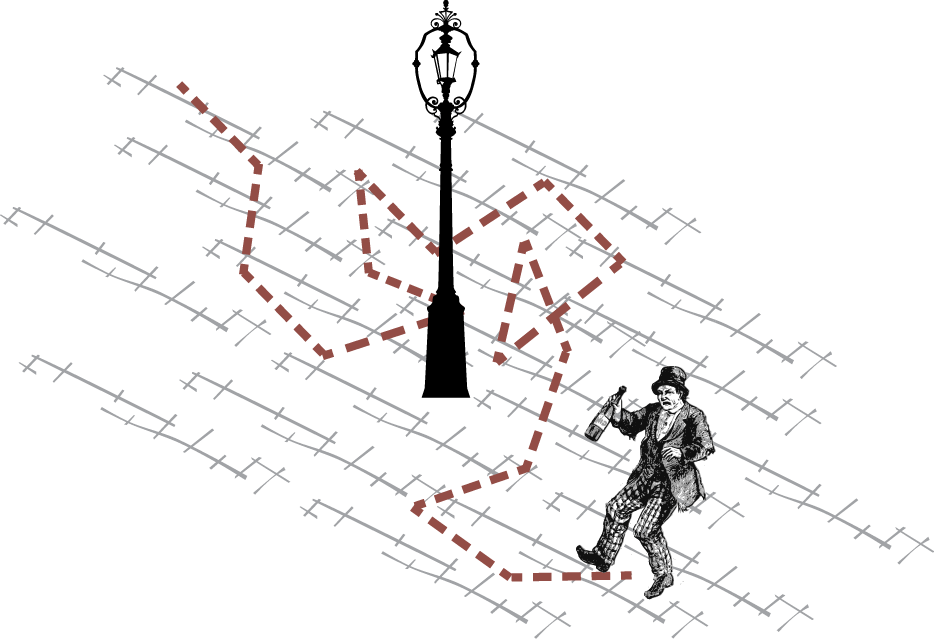
\includegraphics[width=0.99\textwidth]{fig/drunkard}
      \end{center}
    \end{minipage}
    \begin{center}
      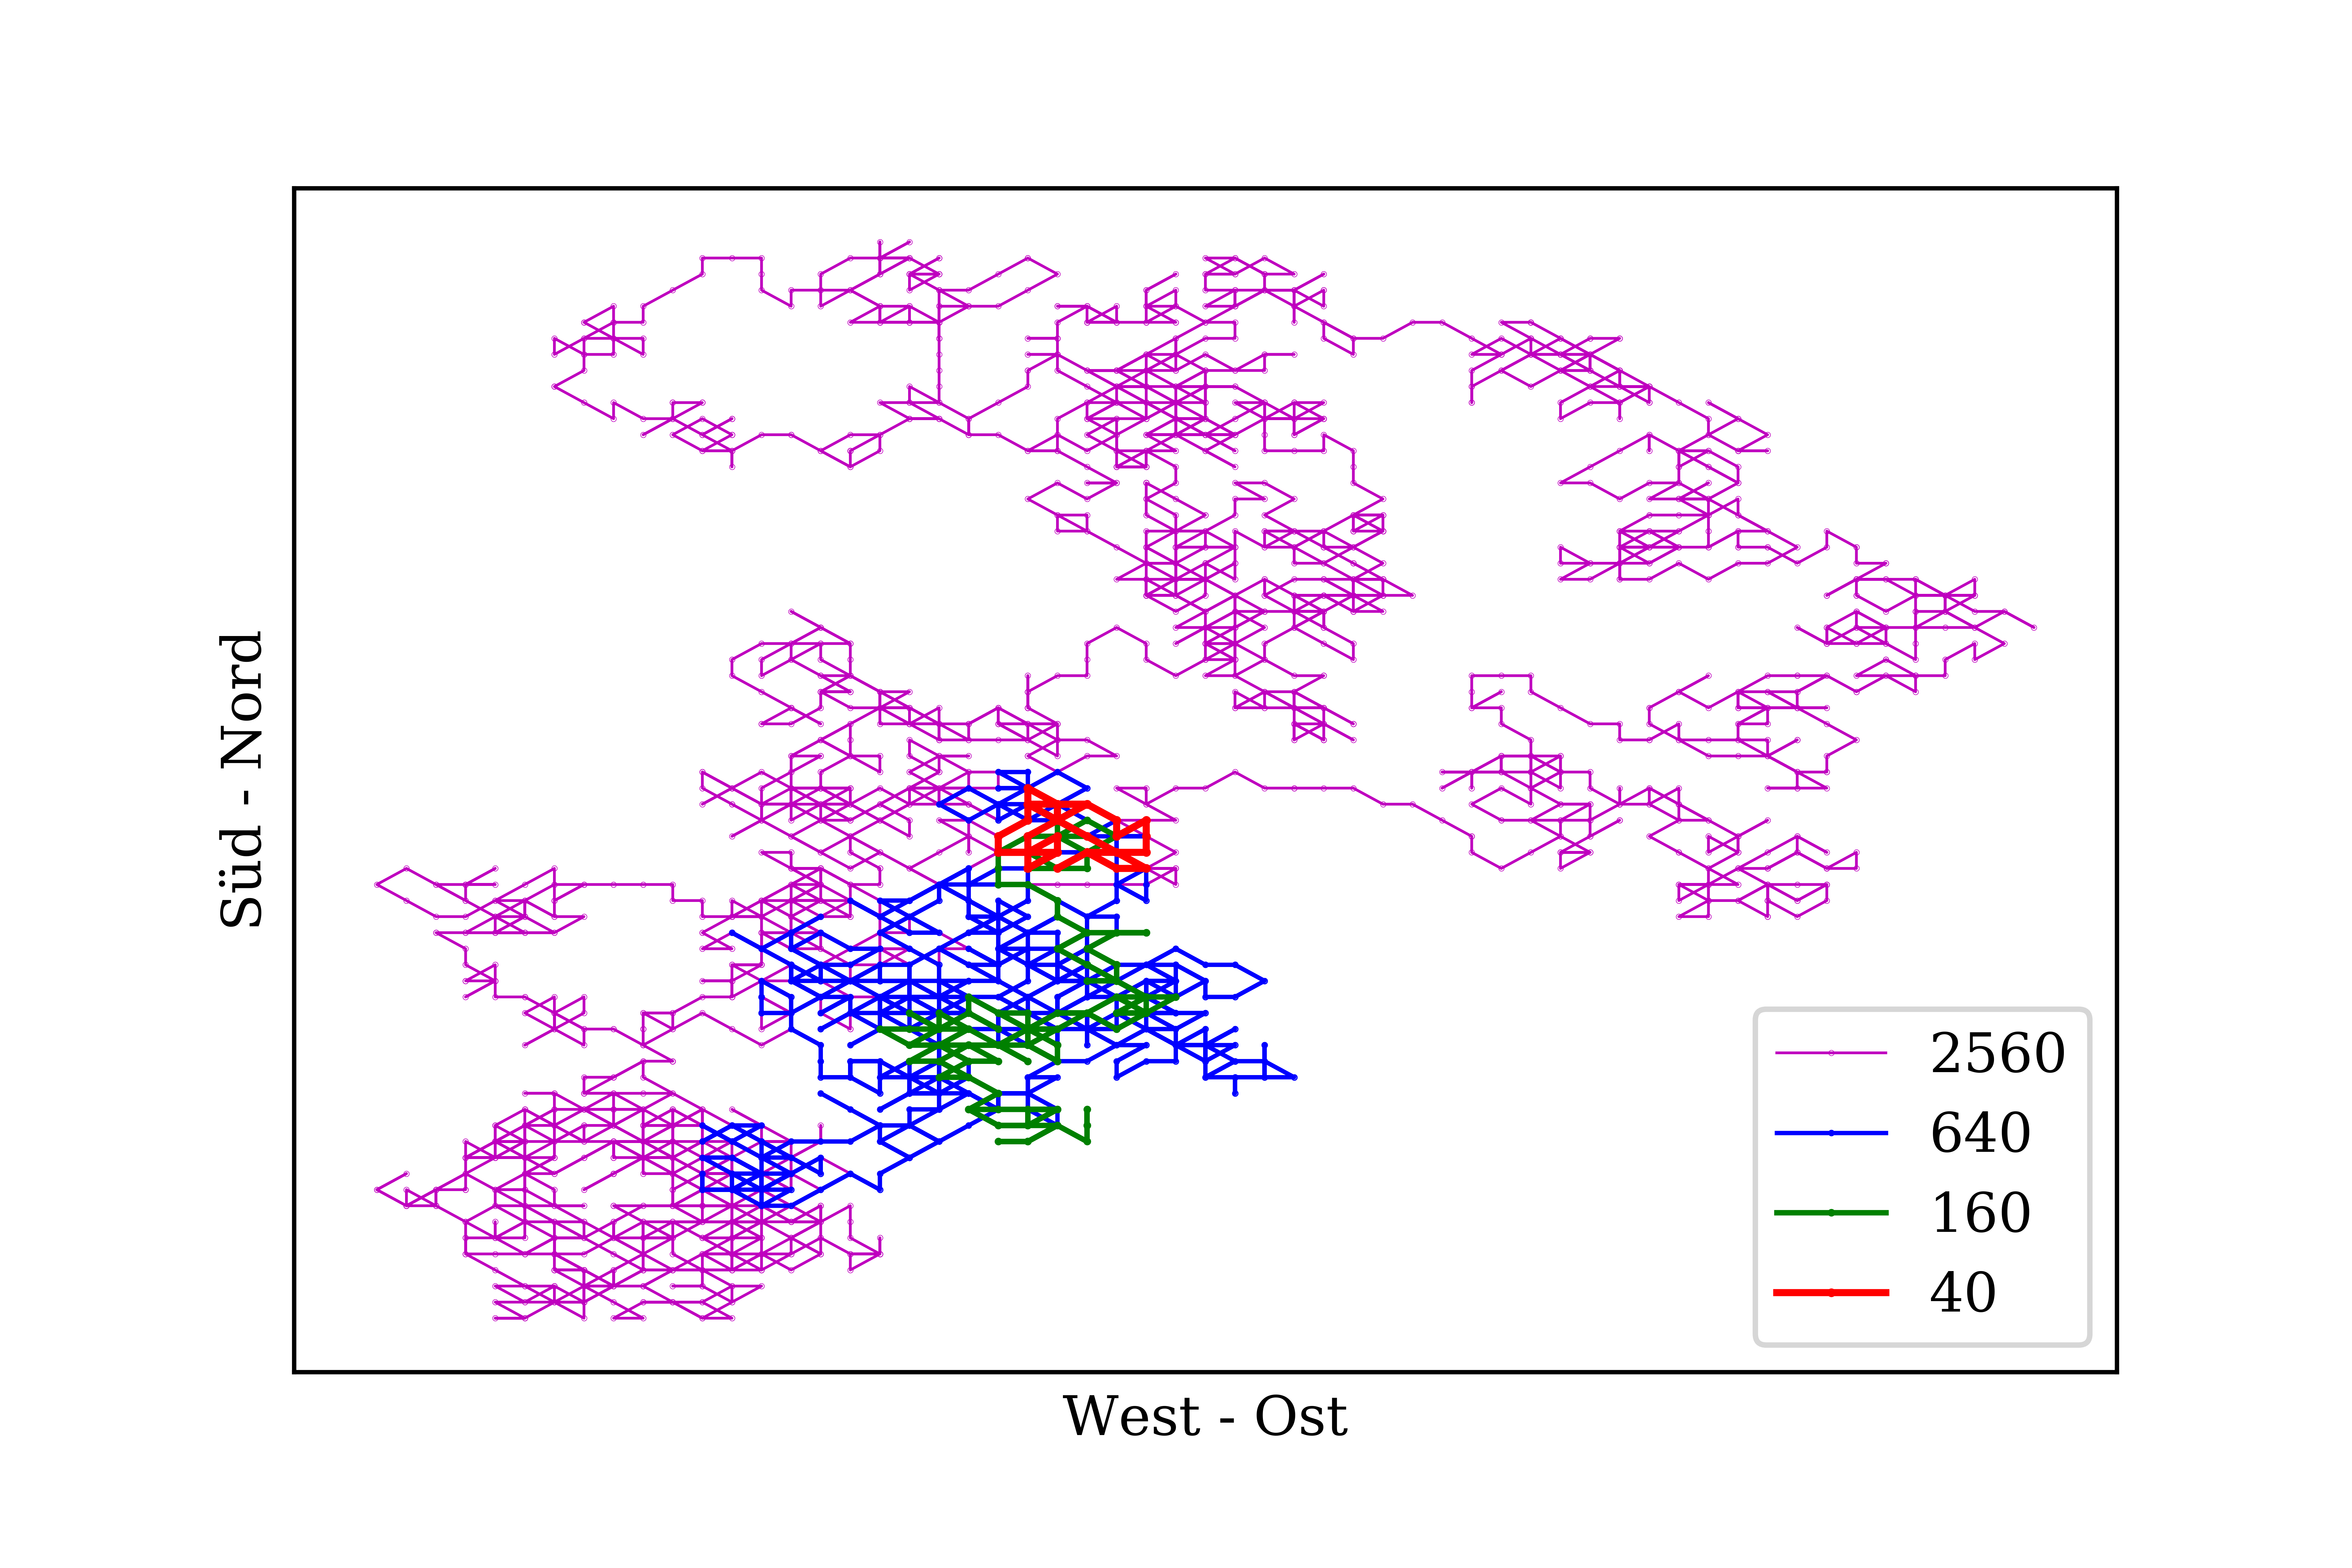
\includegraphics[width=0.9\textwidth]{fig/randomWalkPy}
    \end{center}
    \begin{minipage}[c]{0.7\textwidth}
      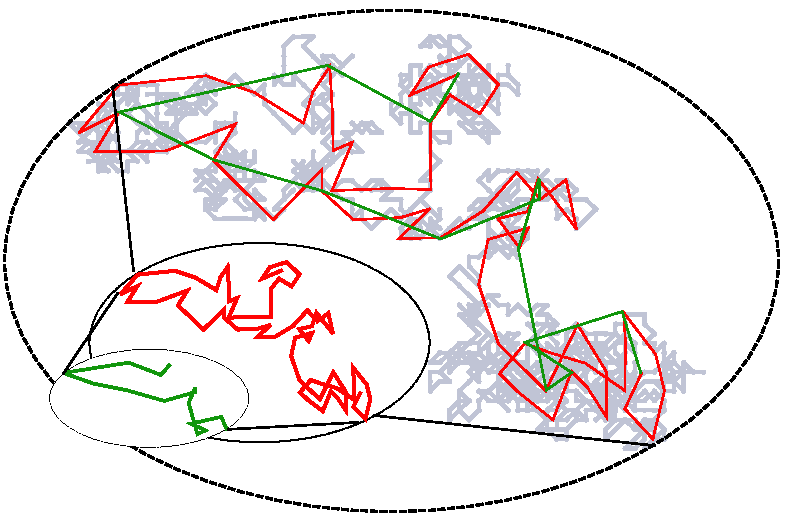
\includegraphics[width=0.95\textwidth]{fig/randomWalkSelfsimiliar}
    \end{minipage}
    \begin{minipage}[c]{0.29\textwidth}
      Teil eines Random Walk ist wieder ein Random Walk\\
      \textcolor{IPForange}{$\Rightarrow$ \textbf{Selbstähnlich}}

    \end{minipage}
    Das sollte man wissen:
    \begin{itemize} \setlength\itemsep{1.1em} \Large
      \item der \textit{Erwartungswert des End-zu-Anfang Abstandes} 
      \begin{align*}
        \langle R \rangle=0
      \end{align*}
      $\Rightarrow$ Bob \textbf{kehrt mit hoher Wahrscheinlichkeit zur Kneipe zurück}
      \item der \textit{Erwartungswert des quaradatischen End-zu-Anfang Abstandes} 
      \begin{align*}
        \langle R^2 \rangle \simeq \text{Anzahl Schritte}
      \end{align*}$\Rightarrow$ viele Schritte $=$ \textbf{immer weitere Wege um den Startpunkt}
    \end{itemize}
  \end{textblock}
  %%--------------------------------------------------------------------------%%

  

\end{myCol}
% ---------------------------------------------------------%
% end the column
% \hspace*{\colsep}%
\hfill
% ---------------------------------------------------------%
% second column
\begin{myCol}
  
%%--------------------------------------------------------------------------%%
  %%--------------------------------------------------------------------------%%
  \begin{textblock}{Selbst\"ahnlichkeit und Dimension von Polymeren - Das Blobmodell}

    \begin{minipage}[c]{0.55\textwidth}
      \begin{itemize} \setlength\itemsep{1.1em} \Large
        \item Lineares Polymer ist langes, kettenartiges Makromolek\"ul
        \item Basiseinheit ist das\\
        \textit{ Monomer} $==$ ein \textit{Schritt}
        \item \textit{Viele} Monomere in zuf\"alliger Richtung aneinander gekettet\\[1.2em]
        $\Rightarrow$ \textcolor{IPForange}{Vorstellung von einem Polymer als sehr langer Zufallsweg}
      \end{itemize}
    \end{minipage}\hfill
    \begin{minipage}[c]{0.41\textwidth}
      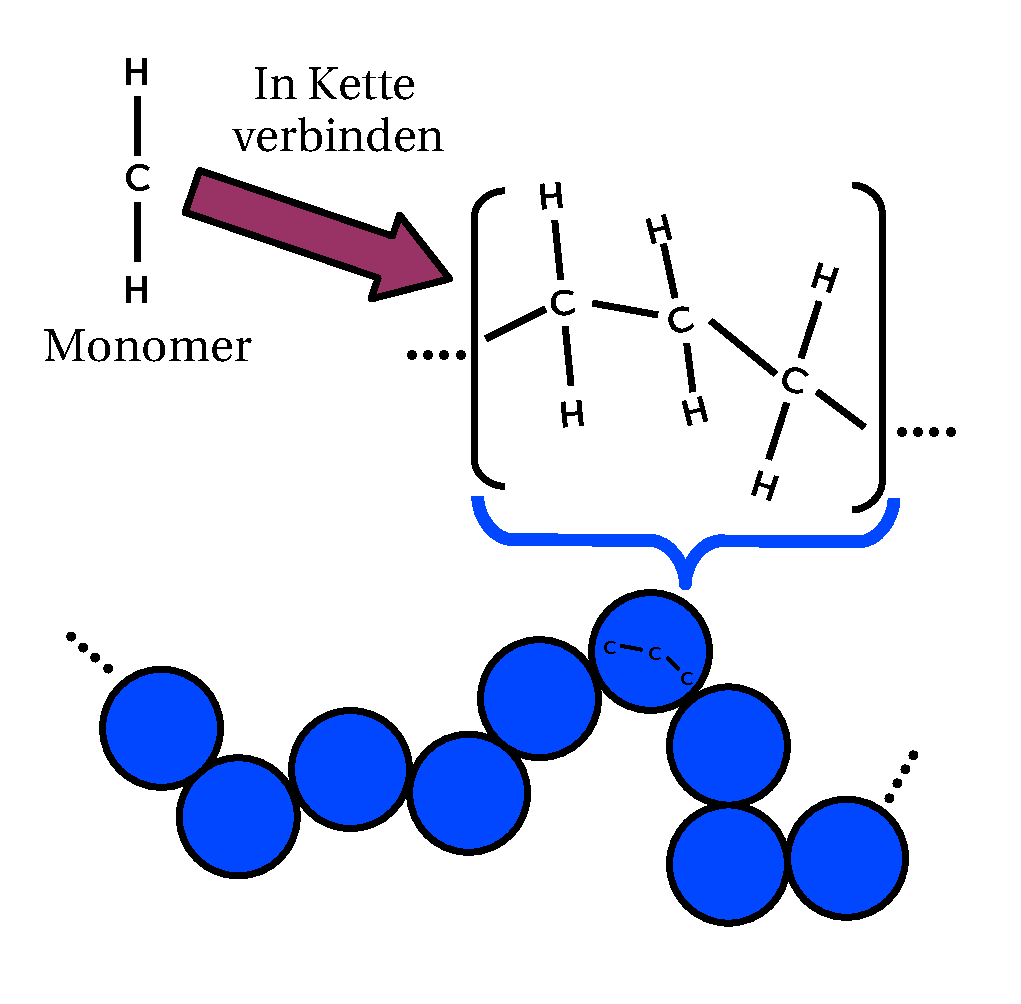
\includegraphics[width=0.75\textwidth]{fig/monchain}
    \end{minipage}
    \vspace*{1cm}
    \begin{center}
      \begin{minipage}[c]{0.2\textwidth}
        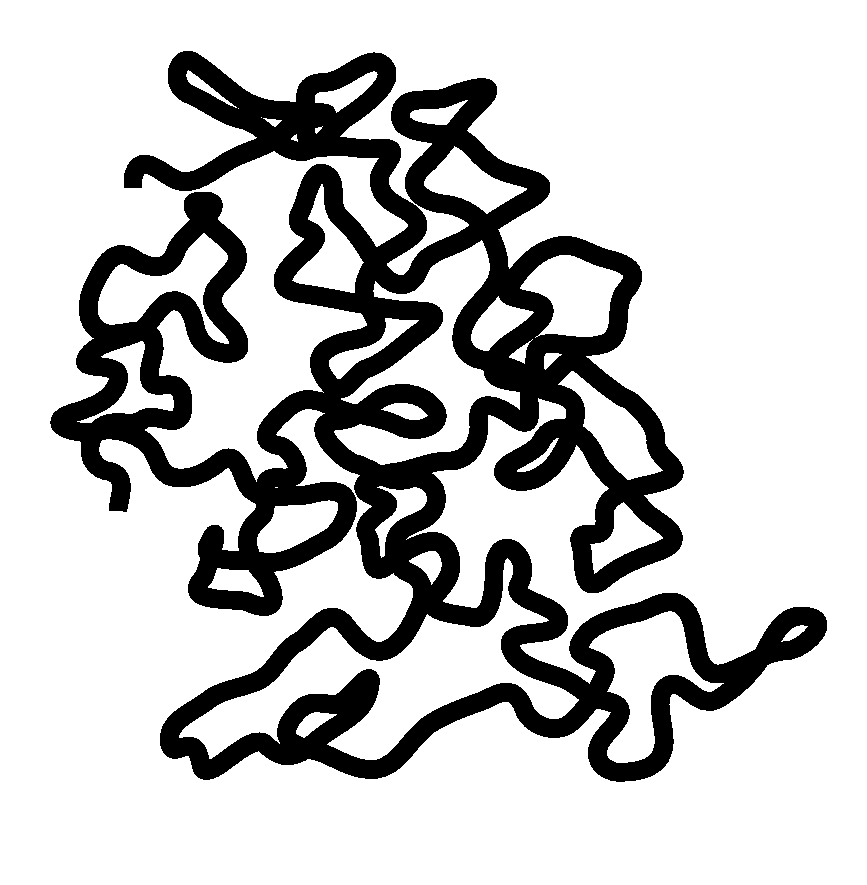
\includegraphics[width=0.94\textwidth]{fig/RW}
      \end{minipage}\hfill
      \begin{minipage}[c]{0.75\textwidth}
        {\Large $\Longrightarrow$ M\"oglicher Zufallsweg eines langen Polymers}\hspace*{1cm}\vspace*{0.5cm}
        \begin{itemize} \setlength\itemsep{1.1em} \Large
          \item Aus der Ferne: regelloses Kn\"auel
          \item Bei wiederholter Vergrößerung: immer ähnliche Struktur\\[1.2em]
          \textcolor{IPForange}{$\Rightarrow$ \textbf{Selbstähnlich}}
        \end{itemize}
      \end{minipage}
    \end{center}\vspace*{0.8cm}
    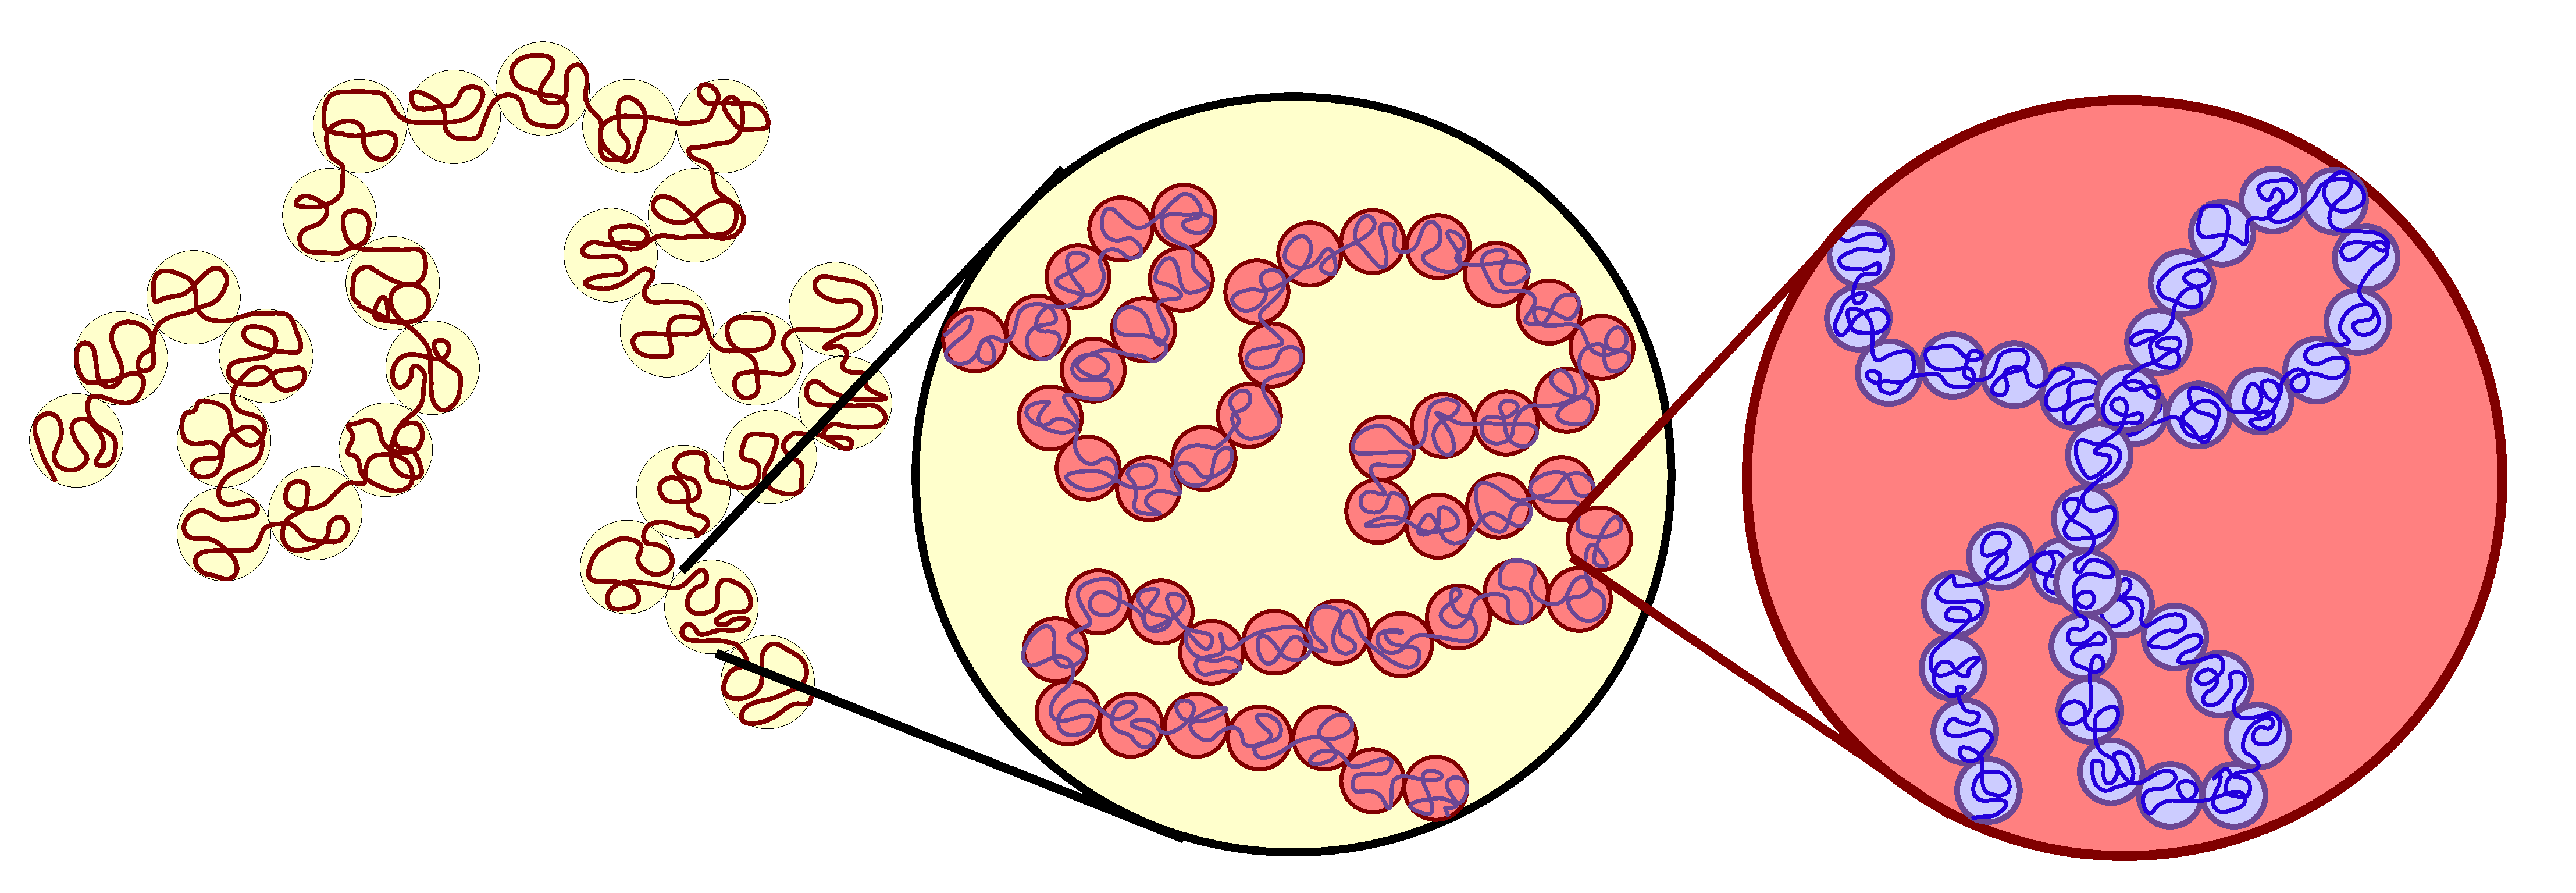
\includegraphics[width=1.05\textwidth]{fig/blob_chain}\vspace*{0.8cm}

    \centerline{ \textbf{\Large Langes Polymer ist \textcolor{IPFred}{selbst\"ahnlich} und besitzt eine \textcolor{IPFred}{Dimension ${ D\neq1} $}}}\vspace*{0.6em}
    \vspace*{2cm}
      \begin{minipage}[c]{0.48\textwidth}\Large
        \textbf{\centerline{Ideales Polymer}}
      \end{minipage}\hfill
      \begin{minipage}[c]{0.48\textwidth}\Large
        \textbf{\centerline{Gutes L\"osungsmittel}}
      \end{minipage}

      \begin{minipage}[c]{0.48\textwidth}\Large
        \vspace*{1.5cm}
        \begin{itemize} \setlength\itemsep{1.1em} \Large
          \item Modellierung als einfacher Zufallsweg
          \item Polymer - eigentlich eine eindimensionale Linie - füllt den Raum wie eine Fläche aus
        \end{itemize}
        \vspace*{4.0cm}
        \begin{flushleft}
          \textcolor{IPFred}{\textbf{ $\Rightarrow$} } gleiche Dimension wie \\ Random Walk
        \end{flushleft}
        \centerline{ \large ${ \boldsymbol{ \rightarrow D=2}}$} 
      \end{minipage}\hfill
      \begin{minipage}[c]{0.48\textwidth}\Large
        \vspace*{1.3cm}
        \begin{itemize} \setlength\itemsep{1.1em} \Large
          \item Modellierung als \textit{Selbstvermeidender Zufallsweg}
          \item Monomere können nicht überlappen\\
          $\rightarrow$ stoßen sich ab\\
          $\rightarrow$ im Vergleich zu Random Walk \textit{quillt} das Polymer
        \end{itemize}
        \vspace*{0.5cm}
        \begin{flushleft}
          \textcolor{IPFred}{\textbf{ $\Rightarrow$} }das Polymer schwillt an bleibt aber selbst\"ahnlich
        \end{flushleft}
      \centerline{ \large ${\boldsymbol{ \rightarrow D\approx1.7}}$}
      \end{minipage}
    \vspace*{4cm}
    \begin{center} \setlength{\baselineskip}{1.2em}
      \textcolor{IPForange}{\textbf{
         \LARGE 
         Ausnutzen der Selbst\"ahnlichkeit und fraktalen\\[0.8cm]
         Dimension erlaubt viele einfache und fundamentale\\[1cm]
         Vorhersagen \"uber das Verhalten von Polymeren} }
    \end{center}
   \end{textblock}
   %%--------------------------------------------------------------------------%%


\end{myCol}%
\end{myTwoColPoster}
\end{frame}
\end{document}


%%% Local Variables:
%%% compile-command: "rake makepdf"
%%% End: